\documentclass[10pt, aspectratio=169]{beamer}

\mode<presentation>{%
    \usetheme{fqs}
    \usecolortheme{fqs}
}

\usepackage{hyperref}
\usepackage{xcolor}
\usepackage{amsmath}
\usepackage{wrapfig}
\usepackage{graphicx}
\usepackage{helvet}
\usepackage[T1]{fontenc}
\usepackage{tikz}
\usetikzlibrary{shapes, arrows, calc, positioning}
\usetikzlibrary{decorations.pathreplacing}
\usepackage{amsmath,amssymb, amsfonts}
\usepackage{lipsum}
\usepackage{verbatim}
\usepackage{datetime}
\usepackage{setspace}

\renewcommand{\familydefault}{\sfdefault}
\renewcommand\mathfamilydefault{}
\newcommand{\colorbf}[1]{{\color{umGreen}\textbf{#1}}}

\newdateformat{dmydate}{%
  \twodigit{\THEDAY}~\monthname[\THEMONTH] \THEYEAR%
}

\title[UM Template]{This \LaTeX Template is Replication of State University of Malang}
\subtitle[Short subtitle here]{Put Your Sub Title Here}
\titlebackground{fqsstyle/assets/gambar-um.jpg}
\author{Firman Qashdus sabil} % Your name
\institute[Universitas Negeri Malang] % Your institution as it will appear on the bottom of every slide, may be shorthand to save space
{\noindent
    \textit{firmanqs@students.ac.id}\par% Your email address
    Group\par
    Position\par
}
\date{\dmydate\today} % Date, can be changed to a custom date

\setbeamersize{text margin left=.05\pdfpagewidth,text margin right=.05\pdfpagewidth}
\begin{document}
%%%%%%%%%%%%%%%%%%%%%%%%%%%%%%%%%%%%
%% Standart title with background image
%%
\maketitle

%%%%%%%%%%%%%%%%%%%%%%%%%%%%%%%%%%%%
%% Title page without background image
%%
{
  \setbeamertemplate{headline}{}
  \begin{frame}
      \begin{tikzpicture}[overlay, remember picture]
          \node[left=1.0cm] at (current page.1){%
              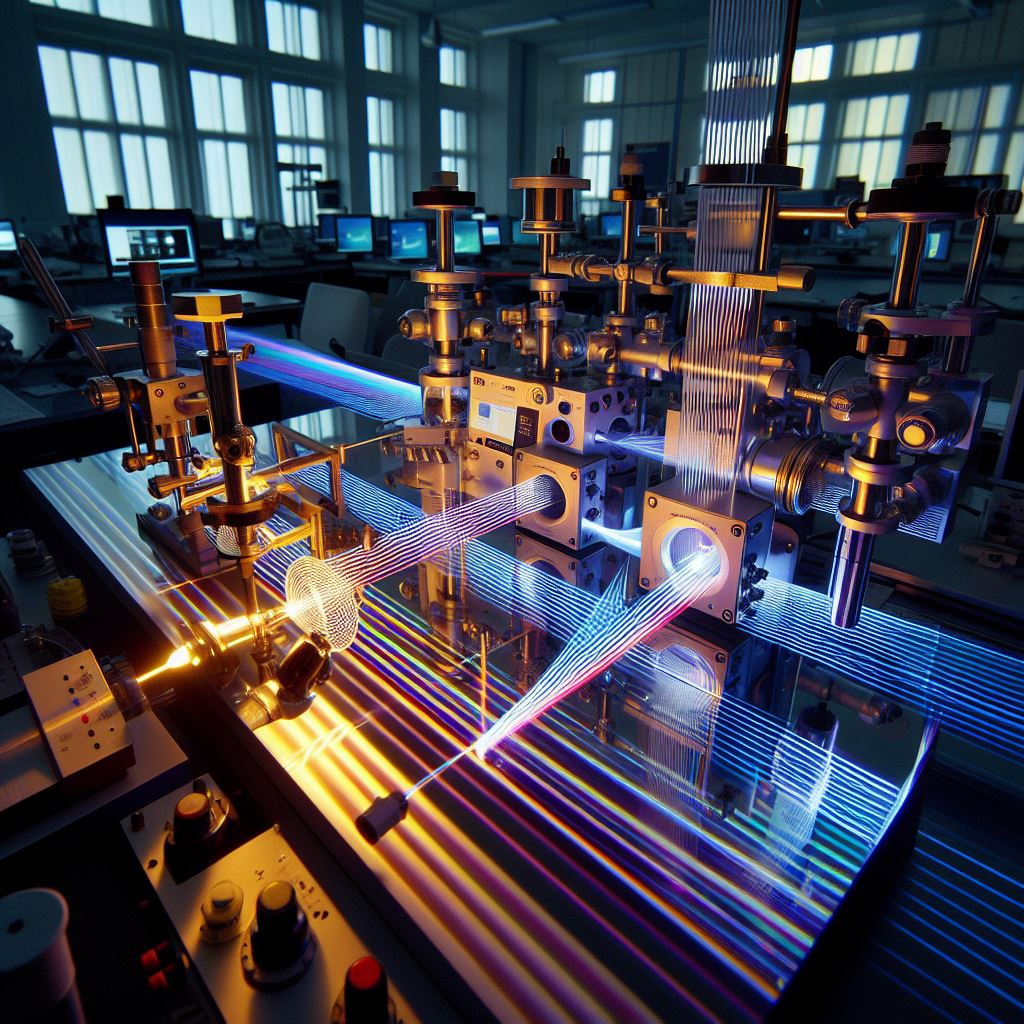
\includegraphics[width=6.5cm]{contents/images/optics-lab}
          };
      \end{tikzpicture}
      \titlepage%
      %%%%%%%%%%%%%%%%%%%%%%
      %% Featured Image
      %%
  \end{frame}
}
\section{Installation}
{
    \setbeamertemplate{headline}{}
    \begin{frame}
        \sectionpage%
        %%%%%%%%%%%%%%%%%%%%%%
        %% Featured Image
        %%
        \begin{tikzpicture}[overlay,remember picture]
            \node[left=2cm] at (current page.2){%
                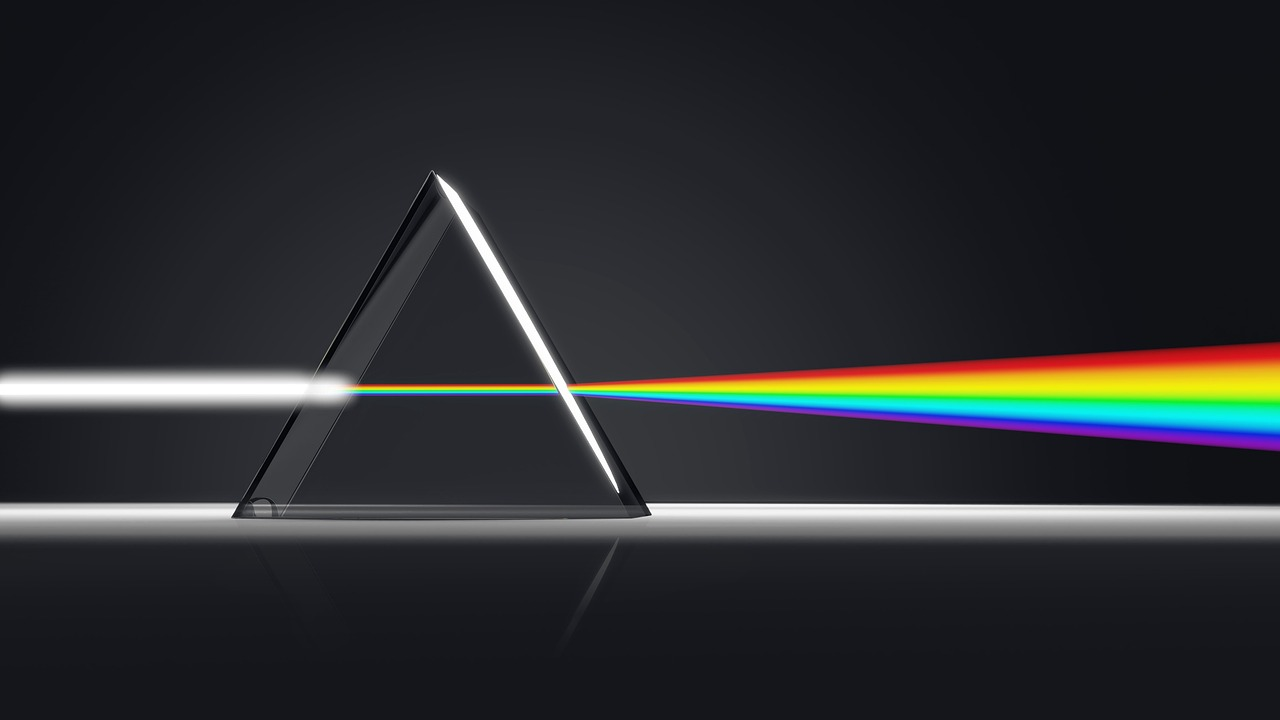
\includegraphics[width=6.5cm]{contents/images/prism-light-dispersion}
            };
        \end{tikzpicture}
    \end{frame}
}
\begin{frame}{Installation}
    To install the the UM beamer theme you need to do the following
    \begin{itemize}
        \item Download 1 the UM beamer package
        \item Download 2 the UM beamer package
        \item Download 3 the broh beamer package
        \item Follow the \href{https://docs.xfel.eu/share/proxy/alfresco/api/node/content/workspace/SpacesStore/92e260f4-e0a7-4463-a812-40a180bd6e75/IN-2012-003-01_LaTeX_User_Guide.pdf?a=true}{\colorbf{European XFEL LaTeX User Guide}} on how to install latex packages.
    \end{itemize}
    \begin{block}{On Linux}
        Extract the package file to\\
        \centerline{\textit{$\sim$/texmf/tex/latex/}}
        and run
        \centerline{ \textit{texhash   $\quad\sim$/texmf/tex/latex/ }}
        in your console.
    \end{block}
\end{frame}

\section{Usage}
\begin{frame}[fragile]{Usage}
    Start your Latex beamer file with:
    \begin{block}{}
\begin{verbatim}
\documentclass[10pt,aspectratio=169]{beamer}
\mode<presentation> {
  \usetheme{UM}
  \usecolortheme{EuXFEL}
}
\end{verbatim}
    \end{block}
\end{frame}

\begin{frame}{Frame Title}
    \begin{itemize}
    \item \lipsum[2][2]
        \begin{itemize}
        \item \lipsum[3][2]
            \begin{itemize}
            \item \lipsum[4][2]
            \end{itemize}
        \end{itemize}
    \end{itemize}

    \begin{block}{Block Title}
        Consider a \colorbf{function} $\rho(r,\phi)$ such that
        \begin{equation}
            \label{eq:1}
            \int_{\gamma} \rho(r,\phi)\, drd\phi=\frac{\pi}{2}
        \end{equation}
    \end{block}
\end{frame}


\begin{frame}{Frame Title}
    \begin{itemize}
    \item \lipsum[2][2]
        \begin{itemize}
        \item \lipsum[3][2]
            \begin{itemize}
            \item \lipsum[4][2]
            \end{itemize}
        \end{itemize}
    \end{itemize}

    \begin{block}{Block Title}
        Consider a \colorbf{function} $\rho(r,\phi)$ such that
        \begin{equation*}
            \mathcal{L} (\theta) = \log \sum_{k=1}^{\lvert Z \rvert} Q(z_k \mid y) \frac{P( z_k,  y \mid \theta)}{Q(z_k \mid y)} \geq \sum_{k=1}^{\lvert Z \rvert} Q(z_k \mid y) \log \frac{P( z_k,  y \mid \theta)}{Q(z_k \mid y)}
        \end{equation*}
    \end{block}
\end{frame}


\begin{frame}{Multiple Columns}
    \begin{columns}[onlytextwidth]
        \begin{column}{0.5\textwidth}
            \lipsum[6][1-4]\\
            \begin{center}
                \def\ry{.6}        % vertical radius outer ellipse
                \def\kry{\ry*.5} % vertical radius inner ellipse
                \def\rx{.3}        % horizontal radius outer ellipse
                \def\krx{\rx*.5} % horizontal radius inner ellipse

                \begin{tikzpicture}[scale=3]
                    % outer ellipse
                    \draw ([shift=(0:{\ry} and \rx)]0,0) arc (0:360:{\ry} and \rx);
                    % hole (inner ellipse)
                    \draw ([shift=(190:{\kry} and \krx)]0,\kry*.25) arc (190:350:{\kry} and \krx);
                    \draw ([shift=(315:{\kry} and \krx)]0,\kry*.25) arc (45:135:{\kry} and \krx);
                \end{tikzpicture}
            \end{center}
        \end{column}
        \begin{column}{0.5\textwidth}
            \begin{enumerate}
                \item \lipsum[6][6]
                \item \lipsum[6][7]
                \item \lipsum[6][8]
                \item \lipsum[6][9]
            \end{enumerate}
            \begin{block}{\centering Something very\\ important!}
                \vspace{-3cm}
            \end{block}
        \end{column}
    \end{columns}
\end{frame}

\end{document}

%%% Local Variables:
%%% mode: latex
%%% TeX-master: t
%%% End:
